\chapter{Evaluation}
\label{sec:eval} 

The 'Evaluation' tab allows adapting/defining requirement-based standards and compliance assessment of said standards. \\

\section{Pre-Requisites \& Limitations}
\label{sec:eval_prereq} 

\begin{itemize}  
\item Target report associations must be set (using \nameref{sec:reconst})
\item At least 1 sector has to be defined (using \nameref{sec:ui_configure_sectors})
\item Usable reference data must exist
\item Usable test data must exist
\end{itemize}
\ \\

While it is possible to manually remove single targets from the evaluation, the usage of correct reference data is paramount for the significance of the evaluation results. \\

\includegraphics[width=0.5cm]{../../data/icons/hint.png} \textbf{Please note that the evaluation feature should not be used as a sole basis for decision making - especially not without manually verifying the evaluation results.}

\subsection{Sector Altitude Filtering}

If sectors with altitude limits are used, please be aware that target reports without a Mode C code can not be filtered by the set limit. Therefore such target reports are assumed to be inside in all 
sectors when inside the defined 2D polygons. \\

The 'inside-sector' check is always performed on the reference data only, therefore it is of importance to only use reference data with existing Mode C code data.

\subsection{Reference Data}

The assumption used in the tool is that the reference data is always correct. Therefore, sub-optimal reference data can cause errors, which will be attributed to the test data in the evaluation. \\

To give a few examples what this could mean:
\begin{itemize}  
\item Wrong 'inside-sector' check results: This might remove valid test data from the evaluation and/or attribute errors to the wrong sector
\item Missing target data in reference: This will remove the test data from evaluation for the time-period of the missing reference data
\item Wrong position in reference: This will cause wrong 'inside-sector' check results and/or cause wrong horizontal position accuracy results
\item Wrong/missing Mode C code in reference: This will cause wrong 'inside-sector' check results
\item Wrong/missing identification in reference: This will cause wrong results in identification requirements
\end{itemize}
\ \\

Also, since target secondary attributes are used in the 'Reconstruct References' task, errors in these attributes might also lead to imperfect data association, which could in turn result in wrong evaluation results in some requirements.

\section{Overview}
\label{sec:eval_overview} 

\begin{figure}[H]
    \hspace*{-2.5cm}
    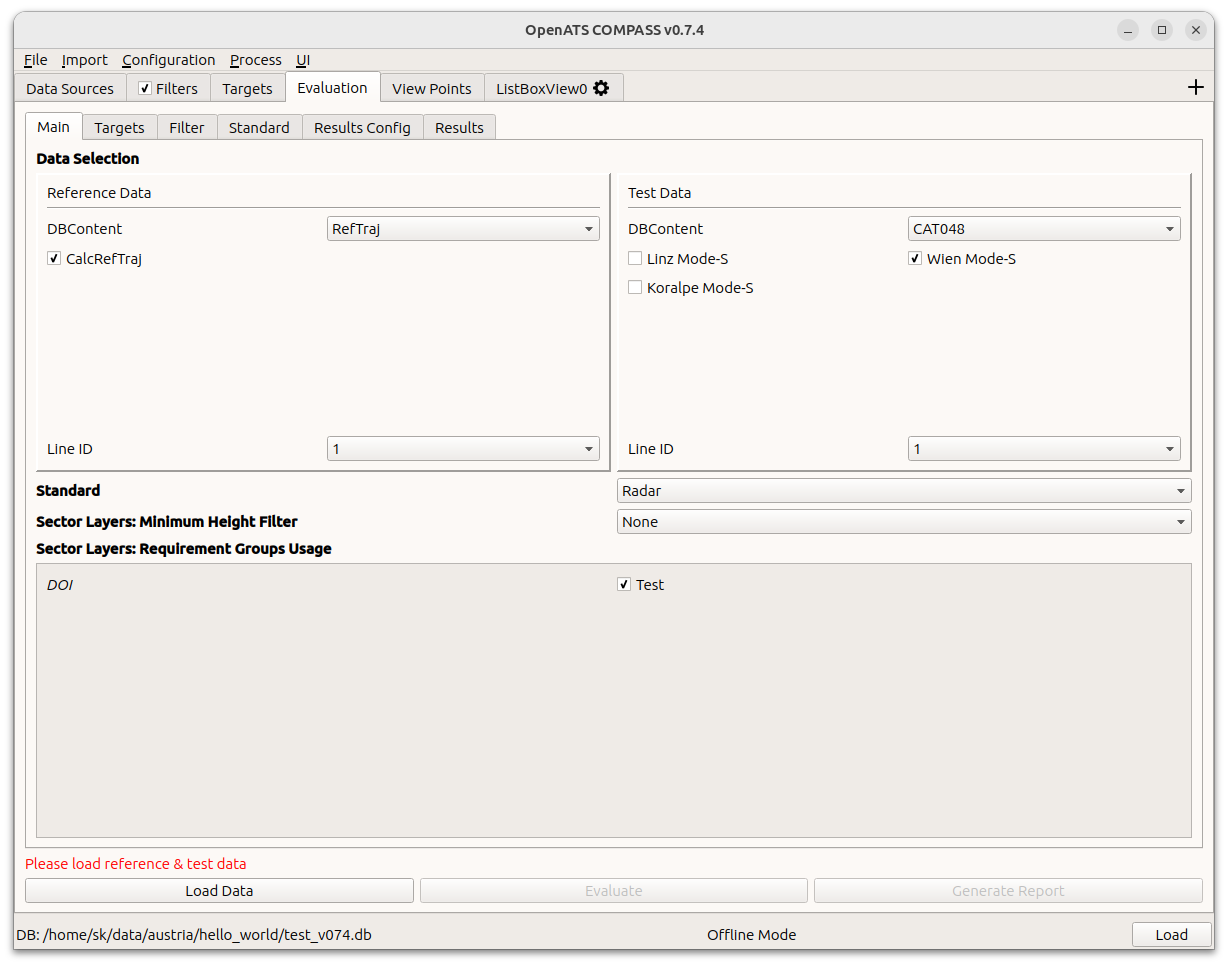
\includegraphics[width=19cm]{figures/eval.png}
  \caption{Evaluation tab}
\end{figure}

At the top, 6 tabs exist:
\begin{itemize}  
\item Main: Main configuration
\item Targets: Table of existing targets in reference / test data (filled after data was loaded)
\item Filter: Filter which data is loaded, by time and/or ADS-B quality indicators
\item Standard: Definition of standards, selection of current standard, configuration of requirements to be checked
\item Results Config: Additional configration for the result generation
\item Results: Evaluation results (created after data was evaluated)
\end{itemize}
\ \\

Below 3 buttons exist:
\begin{itemize}  
\item Load Data: Loads the reference/test data
\item Evaluate: Runs the evaluation of the current standard (available after data was loaded)
\item Generate Report: Generates a report PDF (available when evaluation result exists)
\end{itemize}
\ \\

\section{Configuration}
\label{sec:eval_config} 

\subsection{Main Tab}

\begin{figure}[H]
  \hspace*{-2cm}
    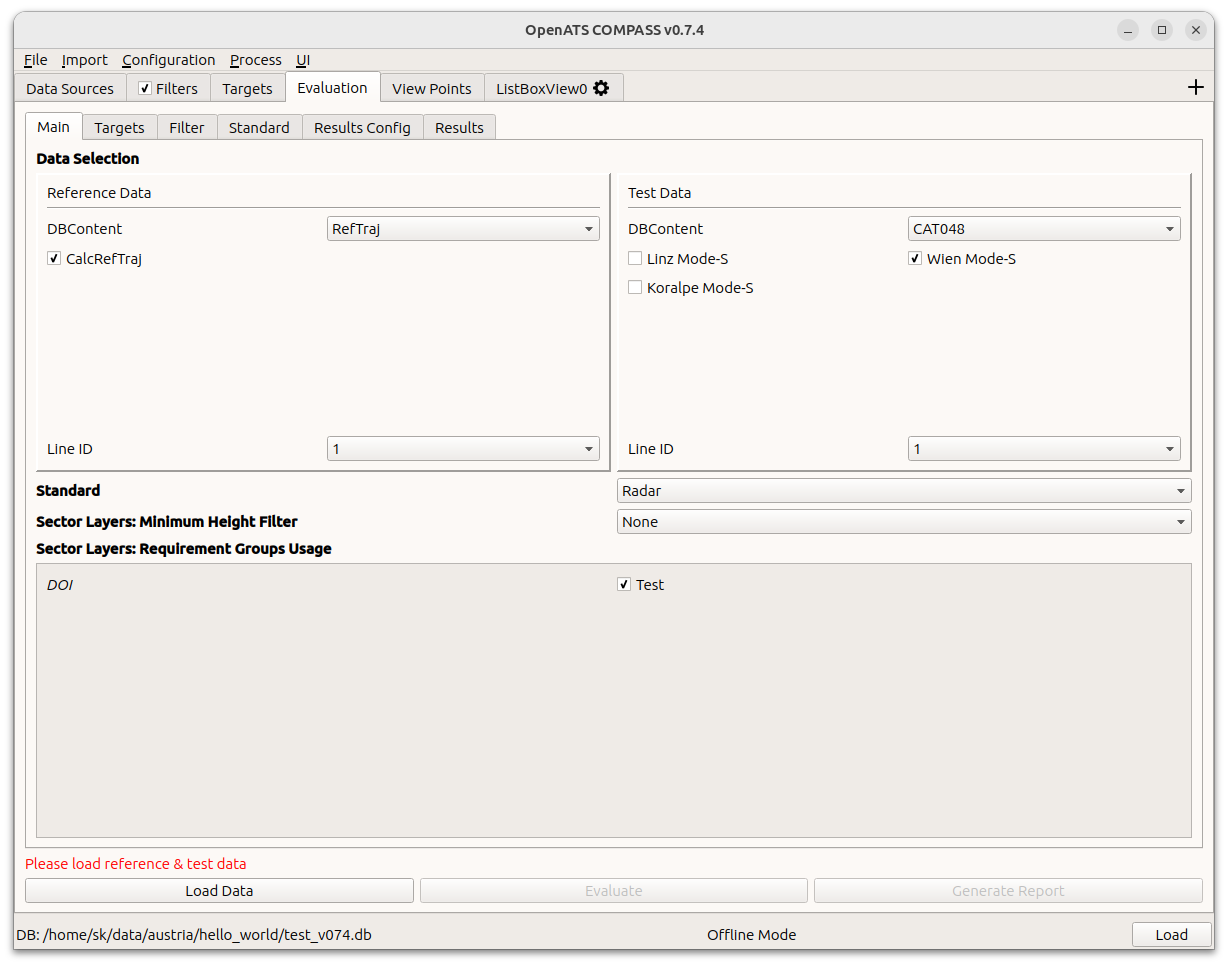
\includegraphics[width=18cm]{figures/eval.png}
  \caption{Evaluation Main tab}
\end{figure}

In the main tab, the main configuration settings can be set. \\

\subsubsection{Data Selection}

At the top, the 'Data Selection' can be performed, by selecting:
\begin{itemize}  
\item Reference Data:
\begin{itemize}  
\item DBContent: Any DBContent existing in the database
\item Data source checkboxes: Which data sources to use
\item Line ID: Which line to use from the data sources
\end{itemize}
\item Test Data:
\begin{itemize}  
\item DBContent: Any DBContent existing in the database
\item Data source checkboxes: Which data sources to use
\item Line ID: Which line to use from the data sources
\end{itemize}
\end{itemize}
\ \\

As noted before, usage of appropriate reference data is of paramount importance. \\

Since 'any' type of data can be selected for evaluation, this allows for the following use-cases:
\begin{itemize}  
\item Tracker as reference, sensor as test data: Evaluation of sensor
\item Tracker as reference, tracker as test data: Evaluation/comparison of different trackers/tracker runs
\end{itemize}
\ \\

Of course it is also possible to use e.g. an imported GPS trail as reference (see \nameref{sec:ui_import_gps}), although this is currently not tested for lack of test data. 
If you might be able to provide such test data, please contact the author. \\

\subsubsection{Standard}
In the center, using the 'Standard' drop-down menu, the current standard can be selected. To create/configure the standard please use the 'Standard' tab.

\subsubsection{Minimum Height Filter}

The option 'Sector Layers: Minimum Height Filter' can be used to select a sector layer, which then serves as a complex minimum height filter.
The selected layer may consist of several sectors with configured minimum altitude, and data which does not lie inside the bounds and above the minimum altitude 
of at least one of the selected layer's sectors will automatically be treated as if residing outside of any evaluation sector. 
The filter thus acts as an additional precondition for data to be regarded by the evaluation.

\subsubsection{Sector Layer/Requirement Mapping}

Below that, the 'Sector Layers: Requirement Groups Usage' allows to define which requirements should be verified for which sector layer. \\

On the left, all existing sector layers are listed, in the shown example:
\begin{itemize}  
\item fir\_cut\_sim: DOI altitude limitation
\end{itemize}
\ \\

For each sector layer, the requirement groups (defined in the Standard tab) can be active/disabled. In the shown example, the existing requirement group 'Mandatory' is active in the sector layer. \\

\textbf{Note}: When selecting a minimum height filter, it usually makes no sense to evaluate requirements in this layer.
All requirement mappings thus should be deselected for this layer (see figure below).

\begin{figure}[H]
  \hspace*{-2cm}
    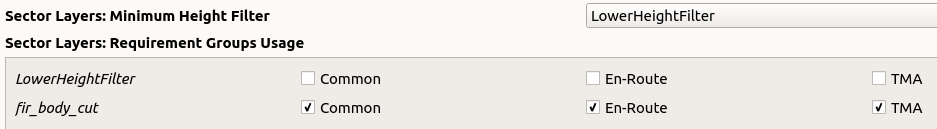
\includegraphics[width=18cm,frame]{figures/eval_unmap_min_height_filter.png}
  \caption{Minimum Height Filter}
\end{figure}

\subsection{Targets Tab}

\begin{figure}[H]
  \hspace*{-2cm}
    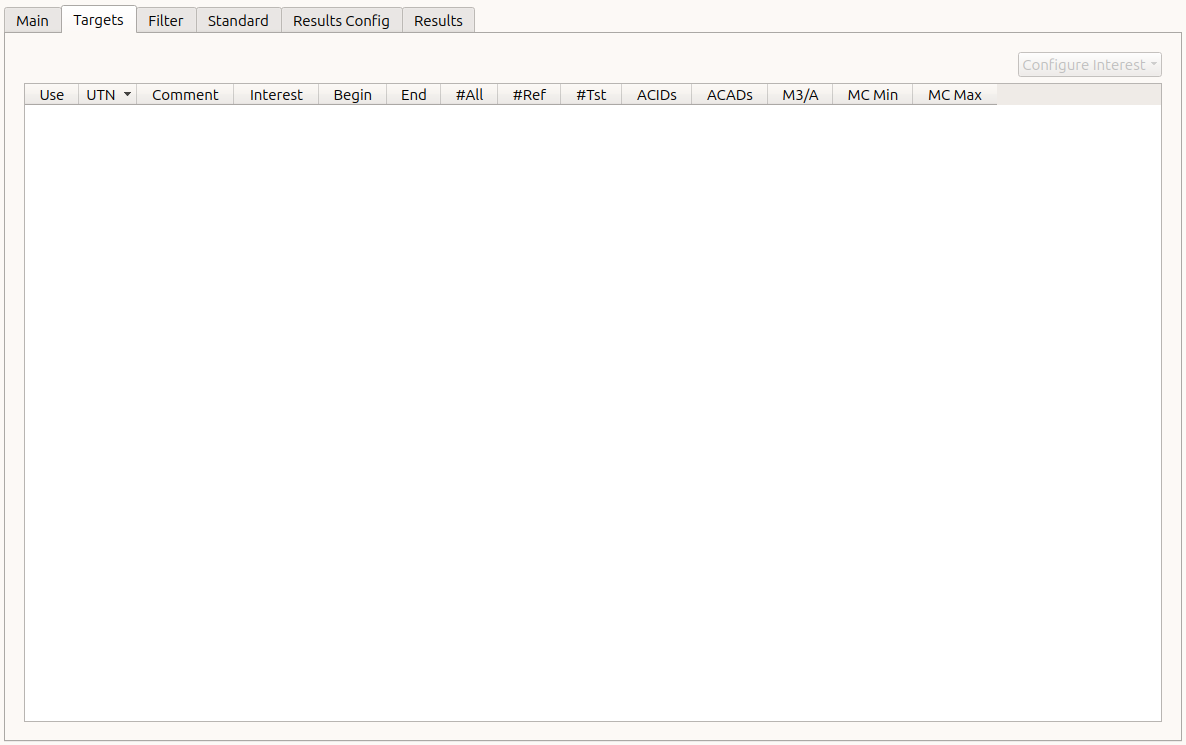
\includegraphics[width=18cm,frame]{figures/eval_targets_empty.png}
  \caption{Evaluation Targets tab}
\end{figure}

Before the data was loaded, the table is empty. Each target (defined by the UTN) is shown in a dedicated row. \\

The following columns exist:

\begin{itemize}  
\item Use: Checkbox defining if the target should be used in the evaluation
\item UTN: Unique Target Number
\item Comment: User comment, can be set with double-click, persisted into database
\item Interest: Score showing how strong a negative impact a target had on all requirement results. Please refer to \nameref{sec:eval_targets_of_interest} for details.
\item Begin: First timestamp of UTN
\item End: Last timestamp of UTN
\item \#All: Sum number of target reports
\item \#Ref: Number of target reports in reference data
\item \#Tst: Number of target reports in test data
\item ACIDs: Mode S aircraft identification(s)
\item ACADs: Mode S aircraft address (hexadecimal)
\item M3/A: Mode 3/A code(s) (octal)
\item MC Min: Mode C code minimum [ft]
\item MC Max: Mode C code maximum [ft]
\end{itemize}
\ \\

Unless otherwise specified, the column content reflects the values from both reference and test data. \\

After loading the data, the table can look as follows:

\begin{figure}[H]
  \hspace*{-2cm}
    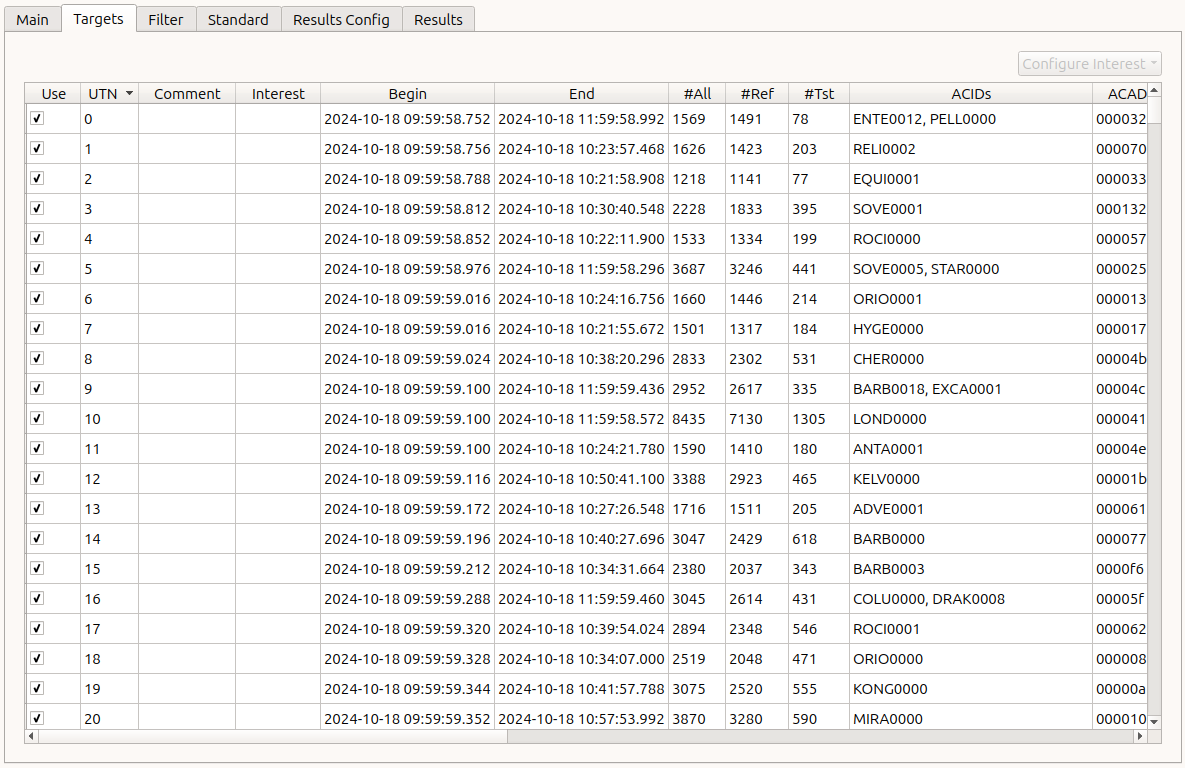
\includegraphics[width=18cm,frame]{figures/eval_targets_loaded.png}
  \caption{Evaluation Targets tab with loaded data}
\end{figure}

After evaluation (and sorting by interest), the table can look as follows:

\begin{figure}[H]
  \hspace*{-2cm}
    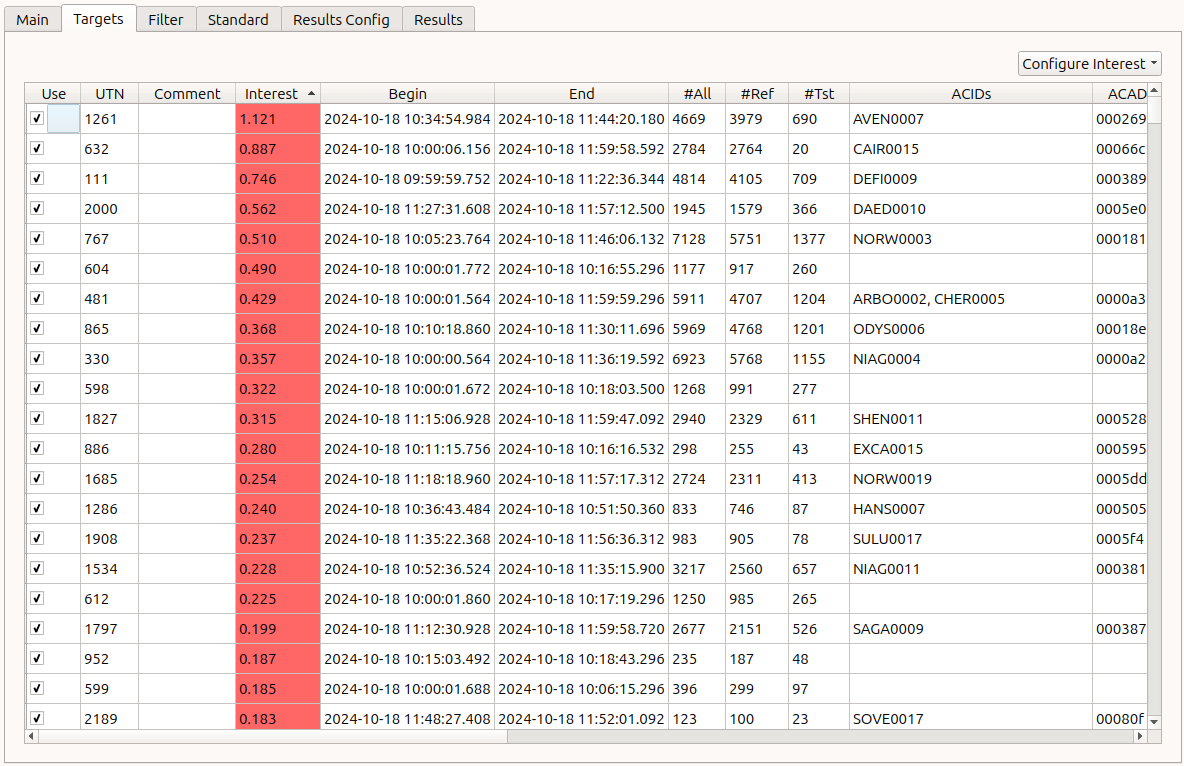
\includegraphics[width=18cm,frame]{figures/eval_targets_eval.png}
  \caption{Evaluation Targets tab with evaluated data}
\end{figure}

\subsection{Filter Tab}

\begin{figure}[H]
  \hspace*{-2cm}
    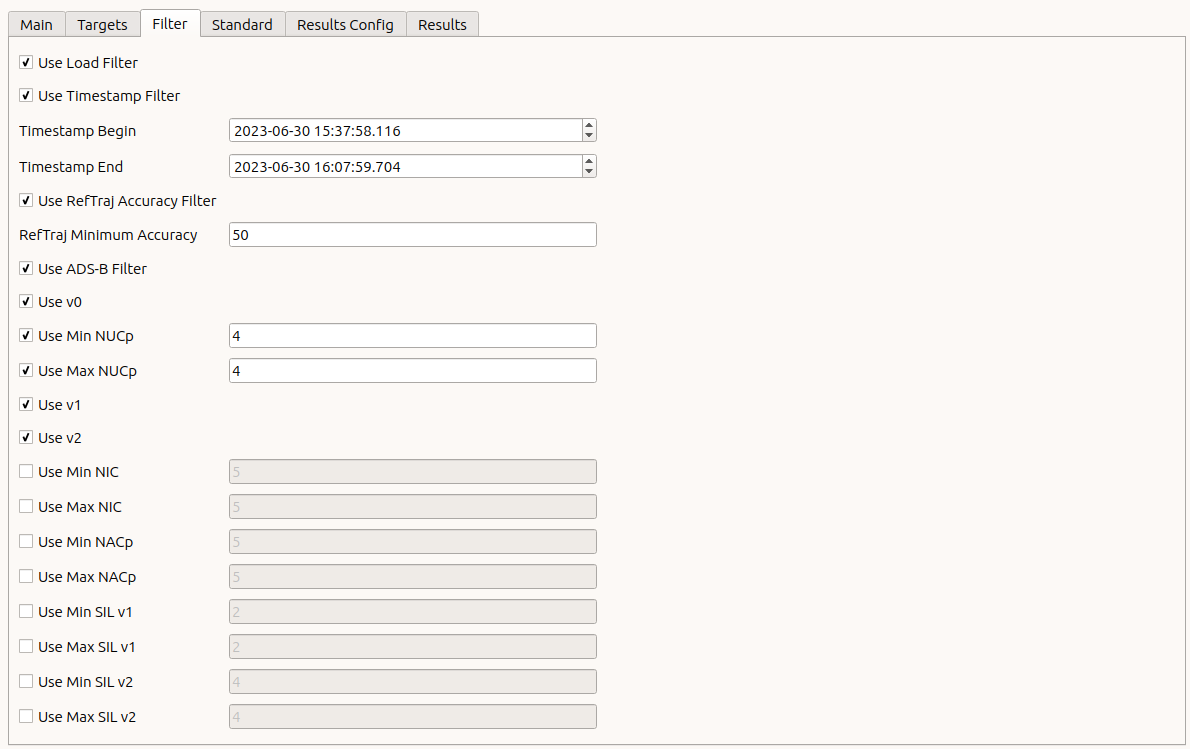
\includegraphics[width=18cm,frame]{figures/eval_filter.png}
  \caption{Evaluation Filter tab}
\end{figure}

In the Filter tab, what data is loaded for evaluation can be filtered \\

Below, the following elements exist:
\begin{itemize}  
\item 'Use Load Filter': Toggles usage of the load filter
\item 'Use Timestamp Filter: Toggles usage of the timestamp filter
\item 'Use RefTraj Accuracy Filter: Toggles usage of the minimum accuracy filter for DBContent RefTraj
\item 'Use ADS-B Filter: Toggles usage of the ADS-B filter
\item 'Use v0: Toggles usage of MOPS Version 0
\item 'Use Min NUCp: Toggles usage of the minimum NUCp value filter
\item 'Use Max NUCp: Toggles usage of the maximum NUCp value filter
\item 'Use v1: Toggles usage of MOPS Version 1
\item 'Use v2: Toggles usage of MOPS Version 2
\item 'Use Min NIC: Toggles usage of the minimum NIC value filter
\item 'Use Max NIC: Toggles usage of the maximum NIC value filter
\item 'Use Min NACp: Toggles usage of the minimum NACp value filter
\item 'Use Max NACp: Toggles usage of the maximum NACp value filter
\item 'Use Min SIL v1: Toggles usage of the minimum SIL v1 value filter
\item 'Use Max SIL v1: Toggles usage of the maximum SIL v1 value filter
\item 'Use Min SIL v2: Toggles usage of the minimum SIL v2 value filter
\item 'Use Max SIL v2: Toggles usage of the maximum SIL v2 value filter
\end{itemize}
\ \\

\subsection{Standard Tab}

\begin{figure}[H]
  \hspace*{-2cm}
    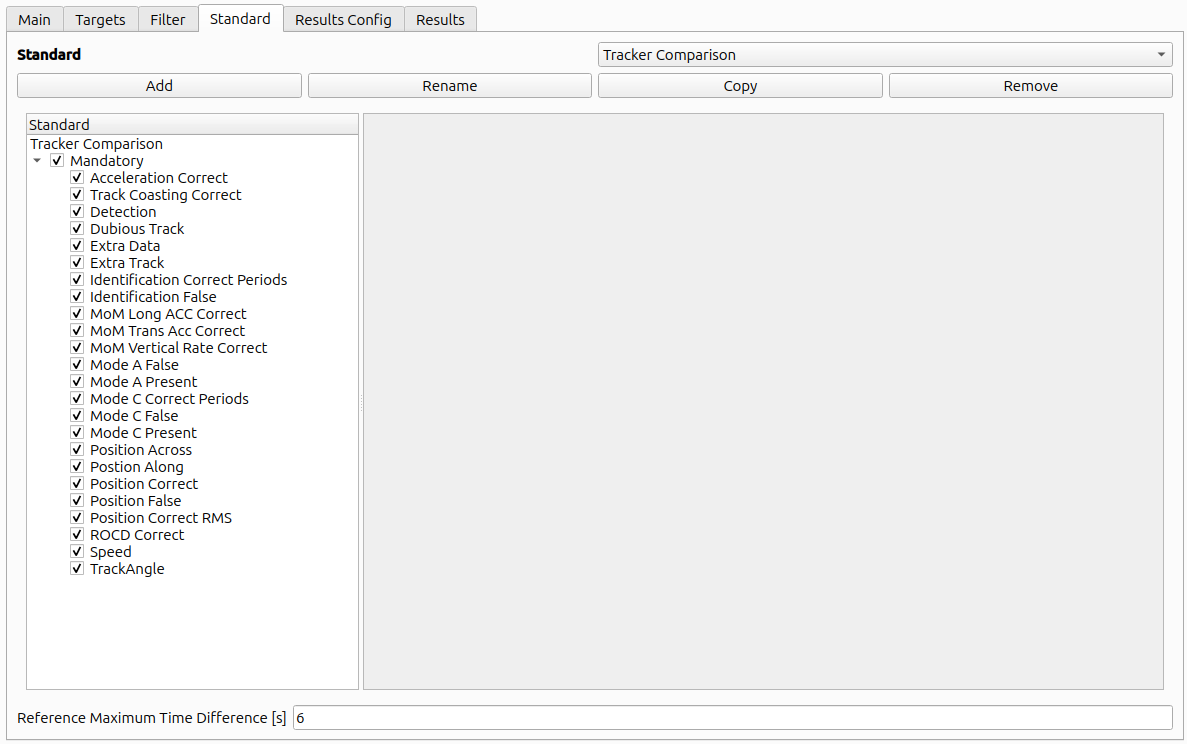
\includegraphics[width=18cm,frame]{figures/eval_standard.png}
  \caption{Evaluation Standard tab}
\end{figure}

In the Standard tab, at the top the current standard can be selected. \\

Below, the following buttons exist:
\begin{itemize}  
\item Add: Add a new standard with a unique name
\item Rename: Rename the current standard
\item Copy: Copy the current standart to a new one
\item Remove: Delete current standard
\end{itemize}
\ \\

At the bottom, the 'Reference Maximum Time Difference [s]' field can be edited to adjust the maximum time difference between reference updates. This value is used to find time-adjacent reference target reports for test target reports. Please adjust this value to e.g. the reference update peroid plus 1 second. \\

Currently, the following standards are (partly) supported:
\begin{itemize}  
\item EUROCAE ED-116 (\href{https://eshop.eurocae.net/eurocae-documents-and-reports/ed-116/}{Link})
\item EUROCAE ED-117/A (\href{https://eshop.eurocae.net/eurocae-documents-and-reports/ed-117a/}{Link})
\item EUROCAE ED-87C/E (\href{https://eshop.eurocae.net/eurocae-documents-and-reports/ed-87c/}{Link})
\item EUROCAE ED-142 (\href{https://eshop.eurocae.net/eurocae-documents-and-reports/ed-142/}{Link})
\item Radar: EUROCONTROL Standard Document for Radar Surveillance in En-Route Airspace and Major Terminal Areas (\href{https://www.eurocontrol.int/sites/default/files/publication/files/surveillance-standard-document-for-radar-surveillance-in-en-route-airspace-and-major-terminal-areas199703.pdf}{Link})
\end{itemize}
\ \\

Please note that, while the EUROCAE ED-117A has been tested using simulator data, the following limitations exist:
\begin{itemize}  
\item In the Stands area, the position accuracy should be calculated using a 5 second position averaging. This is currently not performed, since the averaging method is not specified, and is currently being discussed with users.
\item Some MLAT sensors use a different update rate for non-moving targets. This is currently not regarded, since what constituates non-movement is not (generally) specified, and will lower the probability of detection. 
\end{itemize}
\ \\

Please note that these limitations will be corrected in the near future. \\ 

The other standards have not yet been tested to the fullest degree, which is work in progress.


\subsubsection{Current Standard}

Below that, the current standard is shown. On the left side, a tree-view exists showing:
\begin{itemize}  
\item Standard name
\begin{itemize}  
\item Requirement Group(s)
\begin{itemize}  
\item Requirement(s)
\end{itemize}
\end{itemize}
\end{itemize}
\ \\

\begin{figure}[H]
  \hspace*{-2cm}
    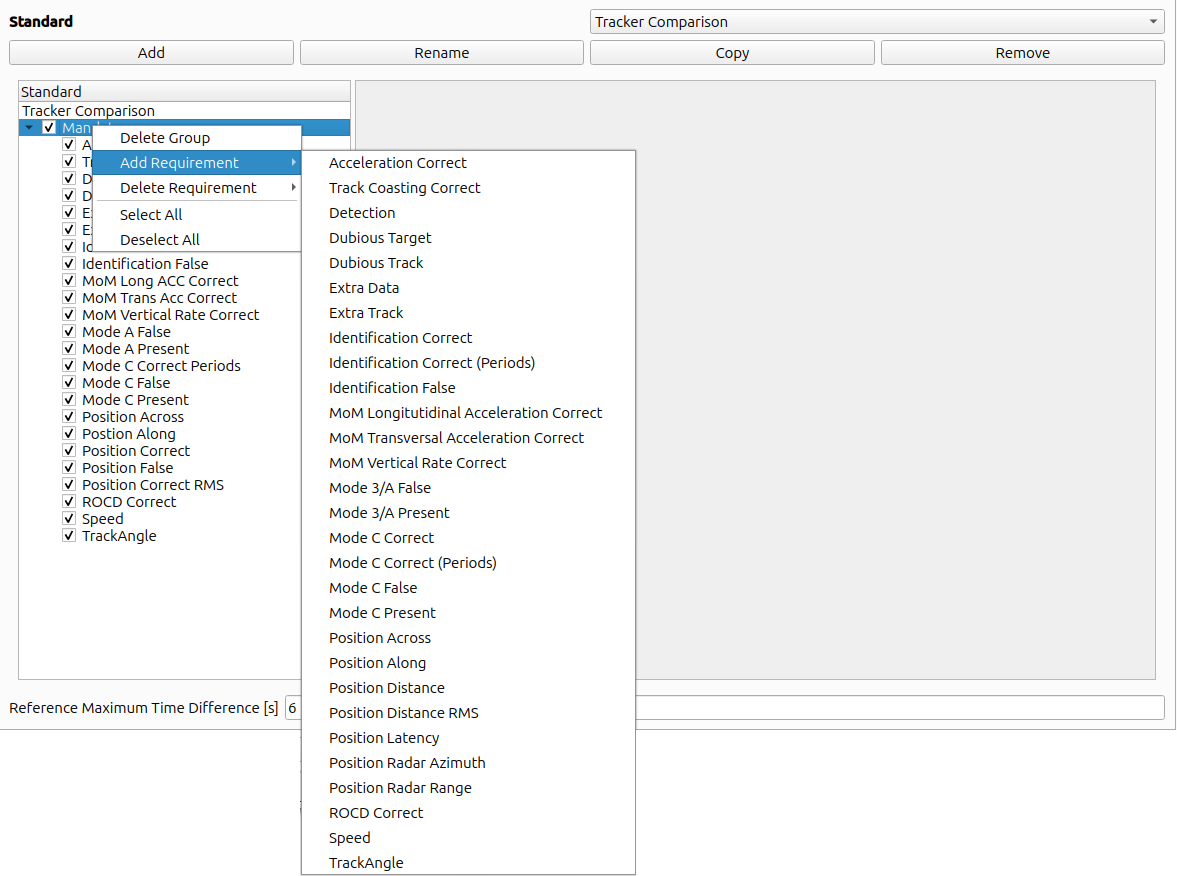
\includegraphics[width=18cm,frame]{figures/eval_standard_add_req.png}
  \caption{Evaluation Standard tab: Add requirement}
\end{figure}

When clicking on the standard name, a menu is shown allowing adding new requirement groups ('Add Group'). \\

When clicking on a requirement group, a menu is shown allowing the following functions:
\begin{itemize}  
\item Delete Group: Delete the selected requirement group
\item Add Requirement: Add a requirement of the selected type
\item Delete Requirement: Delete the selected requirement
\end{itemize}
\ \\

The following requirements exist:

\begin{center}
 \begin{table}[H]
  \begin{tabularx}{\textwidth}{ | l | X |  }
    \hline
    \textbf{Type} & \textbf{Description} \\ \hline
    \nameref{sec:eval_req_accel_correct} & Calculates probability of correct acceleration \\ \hline
    \nameref{sec:eval_req_trk_coast_correct} & Calculates probability of correct track coasting flag \\ \hline
    \nameref{sec:eval_req_detection} & Calculates probability of detection  \\ \hline
    \nameref{sec:eval_req_dubious_targets} & Calculates probability of dubious targets based on physical movement (based on test data only) \\ \hline
    \nameref{sec:eval_req_dubious_tracks} & Calculates probability of dubious tracks from Trackers (based on test data only) \\ \hline
    \nameref{sec:eval_req_extra_data} & Calculates probability of unused test data (based on test data only) \\ \hline
    \nameref{sec:eval_req_extra_track} & Calculates probability of undetected tracks (based on reference data only) \\ \hline
    \nameref{sec:eval_req_id_correct} & Calculates probability of correct secondary identification \\ \hline
    \nameref{sec:eval_req_id_correct_periods} & Calculates probability of correct secondary identification based on UIs \\ \hline
    \nameref{sec:eval_req_id_false} & Calculates probability of false secondary identification \\ \hline
    \nameref{sec:eval_req_mom_long} & Calculates probability of correct MoM Longitudinal Acceleration \\ \hline
    \nameref{sec:eval_req_mom_trans} & Calculates probability of correct MoM Transversal Acceleration \\ \hline
    \nameref{sec:eval_req_mom_vert} & Calculates probability of correct MoM Vertical Rate \\ \hline
    \nameref{sec:eval_req_m3a_false} & Calculates probability of false Mode 3/A code \\ \hline
    \nameref{sec:eval_req_m3a_present} & Calculates probability of Mode 3/A code present \\ \hline
    \nameref{sec:eval_req_mc_correct} & Calculates probability of correct Mode C code \\ \hline
    \nameref{sec:eval_req_mc_correct_periods} & Calculates probability of correct Mode C code based on UIs \\ \hline
    \nameref{sec:eval_req_mc_false} & Calculates probability of false Mode C code \\ \hline
    \nameref{sec:eval_req_mc_present} & Calculates probability of Mode C code present \\ \hline
    \nameref{sec:eval_req_pos_across} & Calculates the probability of the position across error being within a threshold \\ \hline
    \nameref{sec:eval_req_pos_along} & Calculates the probability of the position along error being within a threshold \\ \hline
    \nameref{sec:eval_req_pos_distance} & Calculates the probability of the position error being within or outside a threshold \\ \hline
    \nameref{sec:eval_req_pos_distance_rms} & Calculates the probability of the position error being within or outside an RMS threshold \\ \hline
    \nameref{sec:eval_req_pos_latency}  & Calculates the probability of the position latency being within a threshold \\ \hline
    \nameref{sec:eval_req_pos_radar_azm} & Calculates the probability of the position azimuth error being within or outside a threshold \\ \hline
    \nameref{sec:eval_req_pos_radar_rng} & Calculates the probability of the position range error being within or outside a threshold \\ \hline
    \nameref{sec:eval_req_rocd_correct} & Calculates the probability of correct ROCD \\ \hline
    \nameref{sec:eval_req_speed} & Calculates the probability of the speed error being within or outside a threshold or percentage \\ \hline
    \nameref{sec:eval_req_track_angle} & Calculates the probability of correct track angle \\ \hline
\end{tabularx}
\end{table}
\end{center}
\ \\

If a requirement is clicked, it's configuration widget is shown on the right hand side. \\

Each requirement has the following common attributes:
\begin{itemize}  
\item Type: Type of the requirement
\item Name: Name of the requirement
\item Short Name: Abbreviated name of the requirement
\item Comment: Any text comment, e.g. reference to source document
\item Probability [1]: Probability threshold, as [0,1]
\item Probability Check Type: Probability comparison type for calculated probability against probability threshold
\end{itemize}
\ \\

For detailed information about each requirement please refer to section \nameref{sec:eval_requirements}.

\subsection{Results Config Tab}

\begin{figure}[H]
  \hspace*{-2cm}
    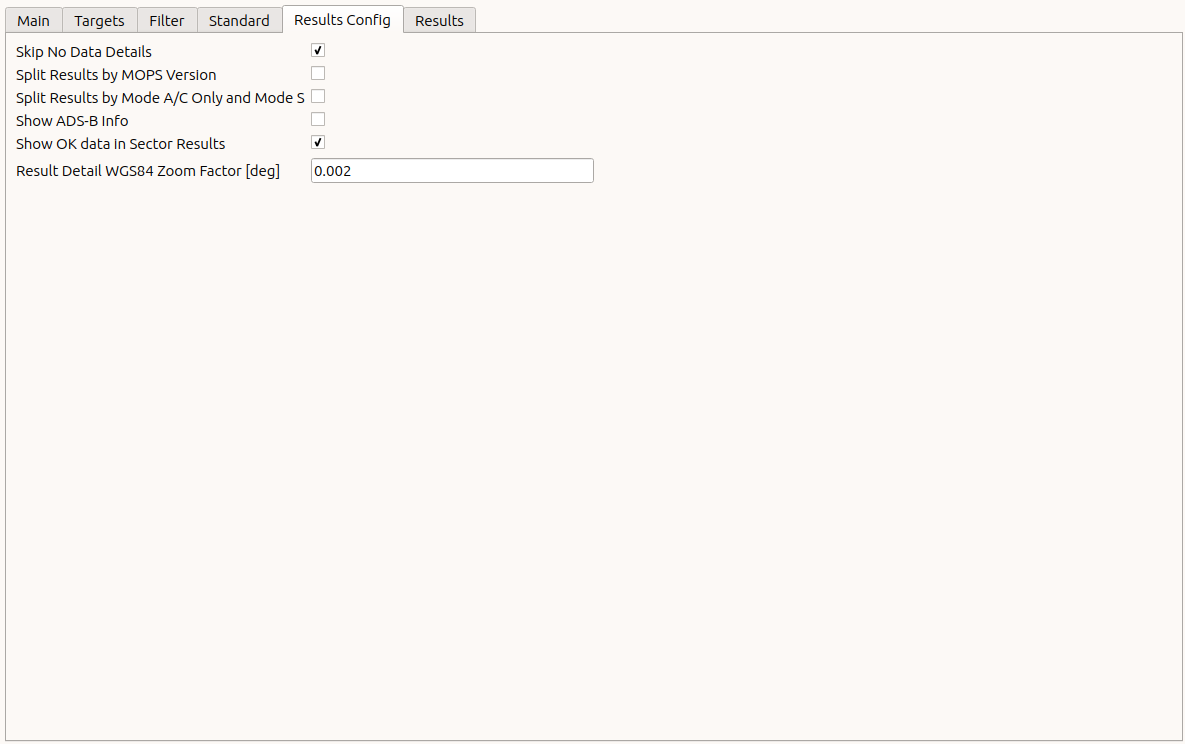
\includegraphics[width=18cm,frame]{figures/eval_results_config.png}
  \caption{Evaluation Results tab}
\end{figure}

The following settings can be used to configure the content of the generated results:
\begin{itemize}  
\item Skip No Data Details: Skip per target report details of no evaluated data existsed (recomended)
\item Split Results by MOPS Version: Split sector aggregations also by ADS-B MOPS Versions (unknown,V0,V1,V2)
\item Split Results by Mode A/C Only and Mode S: Split sector aggregations also by Mode A/C Only and Mode S results
\item Show ADS-B Info: Show ADS-B MOPS Version in results target lists
\item Show OK data in Sector Results: Show also OK markings in sector aggregations (not only errors)
\item Results Detail WGS84 Zoom Factor: Zoom factor in Geographic View for target report details
\end{itemize}
\ \\

\subsection{Results Tab}

\begin{figure}[H]
  \hspace*{-2cm}
    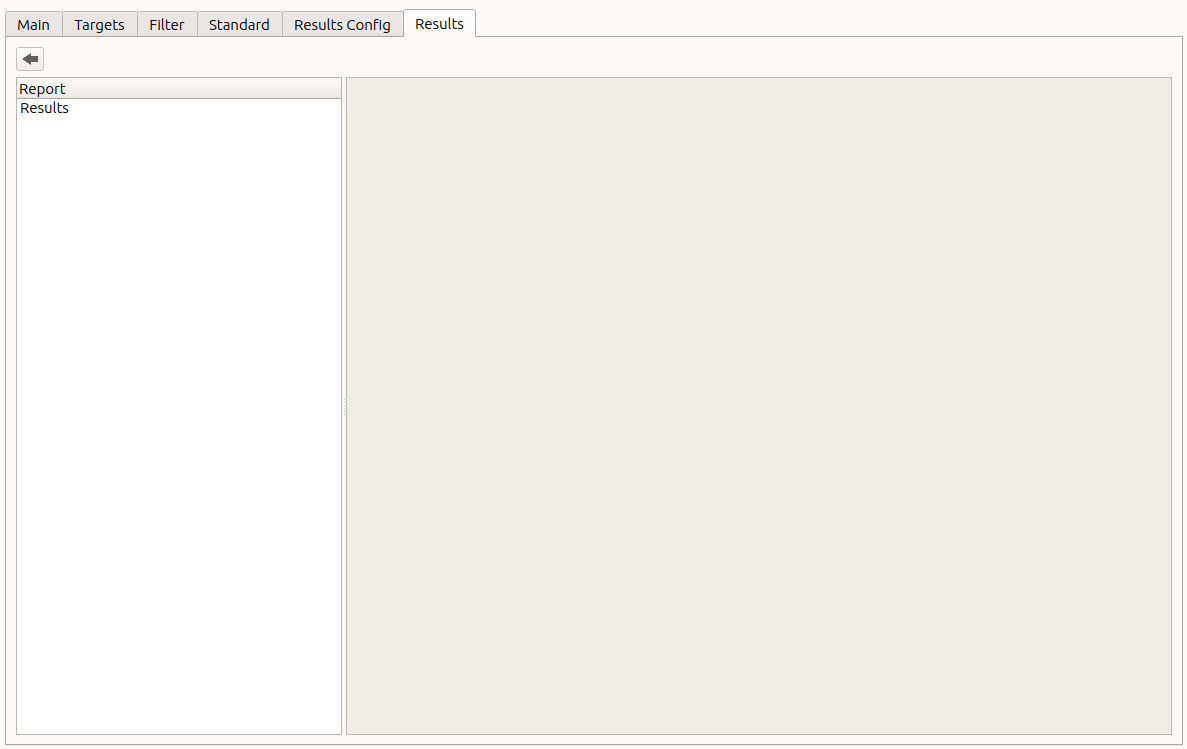
\includegraphics[width=18cm,frame]{figures/eval_results_empty.png}
  \caption{Evaluation Results tab}
\end{figure}

Before the data was evaluated, the results are empty.\\

There are several levels of detail for the results, and each sub-result is shown in a tree-view on the left side, grouped into sections. Using this tree-view, the results can be "navigated", and the currently selected results contents are shown on the right side. \\

More details will be described in the following section \nameref{sec:eval_inspect}.

\section{Running}
\label{sec:eval_run} 

\subsection{Load Data}
\label{sec:eval_run_load} 

After the wanted configuration (in the Main tab) has been set, the 'Load Data' button can be clicked. This results in the reference/test data being loaded, after which a post-processing will be performed. \\

Please note that the post-processing step uses all available cores on the CPU.

\begin{figure}[H]
  \centering 
    \includegraphics[width=8cm]{figures/eval_post.png}
  \caption{Evaluation: Post-processing after loading}
\end{figure}

The post-processing pre-calculates only which reference target reports can be used for direct comparison for specific test target reports. \\

Therefore, please note that re-loading the data is only required when changes to the reference/test data settings in the Main tab have been made. Changing requirements or removing targets from evaluation does not require re-loading. \\

After the loading and the post-processing have been performed, all targets are shown in the Targets tab.

\begin{figure}[H]
  \hspace*{-2cm}
    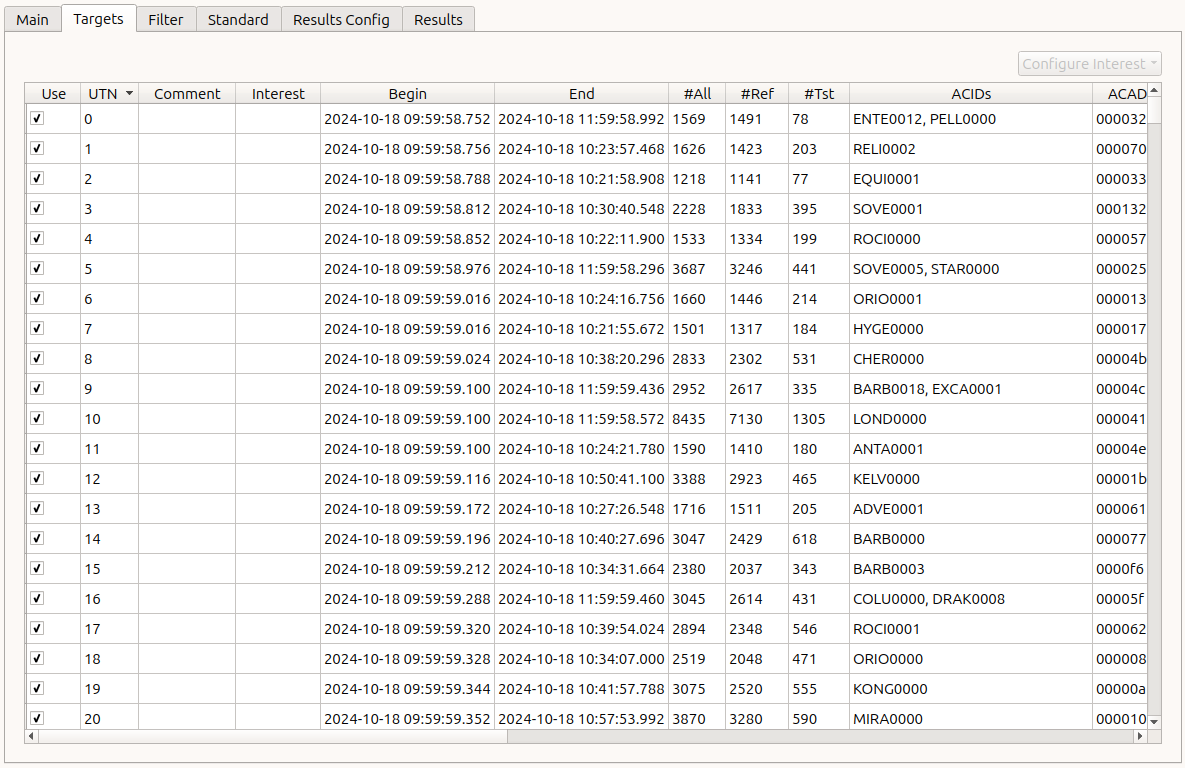
\includegraphics[width=18cm,frame]{figures/eval_targets_loaded.png}
  \caption{Evaluation Targets tab after loading}
\end{figure}
\ \\

Please note that the difference to the main 'Targets' tab list consists in only evaluation targets being shown - i.e. only targets which are present in the currently selected reference / test data.

\subsection{Filtering Targets}
\label{sec:eval_filter_targets} 

The Targets tab is useful for removing certain targets from the evaluation ('Use' checkbox) and inspecting already removed ones. 

Single rows can be selected by clicking on them, which triggers a loading process showing this exact target (with all associated data) in the available Views. Please note that this does not require re-loading the evaluation data, but can be used at all times during the evaluation. \\

To remove targets with certain parameters (e.g. primary-only, black-whitelisting, always low Mode C, ...) please refer to section \nameref{sec:ui_target_filtering}.

\subsection{Evaluation}
\label{sec:eval_run_eval} 

After the data was loaded, the configuration relating to current standard, requirements and sector/requirement group usage can be adapted. After that, the evaluation can be (re-)run using the 'Evaluate' button. \\

This will trigger evaluation of the requirements in all sectors (as configured). The requirement values will be calculated for each target (whether to be used or not). Then, for each requirement and sector, the results are summed-up as per-sector average (if target should be used). \\

Please note that the post-processing step uses all available cores on the CPU.

\begin{figure}[H]
  \centering 
    \includegraphics[width=10cm]{figures/eval_eval_status.png}
  \caption{Evaluation: Running evaluation status}
\end{figure}

The results are then shown in the Results tab.

\subfile{eval_inspect}

\section{Generate Report}
\label{sec:eval_report}

Using the "Export PDF" button, a PDF can be generated. A PDF can only be generated if a Latex environment is installed on the workstation, as described in \nameref{sec:appendix_latex}.

\begin{figure}[H]
    \includegraphics[width=14cm]{figures/eval_report.png}
  \caption{Evaluation results: Generate report dialog}
\end{figure}

At the top, the following configuration options exist:

\begin{itemize}  
\item Report Path: Directory to which the report will be written.
\item Report Filename: Filename of the report, to be created in the report path. File extension must be '.tex'.
\item Change Location: Button to set the report path and filename.
\item Author: Author string, is added to the first page of the report.
\item Abstract: Abstract string, is added to the first page of the report.
\item Include Per-Target Details: Whether to include the per-target details.
\item Include Per-Target Target Report Details: Whether to include the per-target target report details.
\item Wait on Map Loading: When Geographic View screenshots are created, some maps require downloading terrain from the Internet.  This option enables to wait on completion of such activities, to generate high-quality screenshots. Disable only when operating on cached maps without an Internet connection.
\item Run PDFLatex: Automatically runs the pdflatex compile process, immediately creating a PDF after finished export. Is disabled if command could not be found.
\item Open Created PDF: Automatically opens the created PDF. Is disabled if pdflatex command could not be found.
\end{itemize}
\ \\

Please \textbf{note} that the two 'Include ... Details' options can produce very large PDF reports (10.000+ pages), and may even overload the Latex sub-system (will result in 'TeX capacity exceeded, sorry' error). It is therefore recommended to only activate these options for small datasets with very few sector layers. \\

The 'Run' button startes the export process. At the bottom, status information and a cancel button exists. \\

To run the export process, click the 'Run' button.

\begin{figure}[H]
    \includegraphics[width=14cm]{figures/eval_report_status.png}
  \caption{Evaluation results: Generate report in progress}
\end{figure}

If the export process was sucessful, the dialog is closed automatically. The report Latex file was written into the report directory, with screenshots in the 'screenshots' subfolder. If the respective options were set, a PDF was automatically generated and is opened using the default PDF application. \\

If a Latex error ocurred, a message box with the error message is shown. If the 'TeX capacity exceeded, sorry' error is shown, disable one or both of the 'Include ... Details' options.\\

Please note that the generated report can of course be edited by the user and re-generated using pdflatex, which allows for better customization options (adding e.g. details, corporate identity etc.).

\subfile{eval_requirements}
